\begin{surferPage}[Chmutov-Octic]{A Chmutov Octic}
    An eye-catching feature of Chmutov's octic $\text{Chm}_{d}, \ d=8,$
    is its symmetry.
    This can also be seen by inspecting the equation:
    \[\text{Chm}_{d}\colon T_d(x) + T_d(y) + T_d(z) + 1 = 0,\]
     where $T_d$ is the so--called Tchebychev polynomial (left picture).
    The curve $T_8(x)+T_8(y)=0$ is depicted on the right:
    
     \begin{center}
      \begin{tabular}{c@{\quad}c}
        \begin{tabular}{c}
          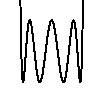
\includegraphics[height=1.75cm]{./../../common/images/Tcheb_008.pdf}
        \end{tabular}    
        &
        \begin{tabular}{c}
          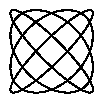
\includegraphics[height=1.75cm]{./../../common/images/Tcheb_2d_008.pdf}
        \end{tabular}    
      \end{tabular}
    \end{center}
    \vspace{-0.3cm}
    The step from these pictures to the shape of the surface in the
    interactive picture is not very long.


These equations where given by S.V.\ Chmutov in the early 80s.
    At that time, they constituted the world record for $\mu(d)$ most $d$.
    In the 90s, Chmutov improved his own record, and in 2005, S.~Breske,
    O.~Labs and D.~van~Straten adapted this construction to yield real
    surfaces with only real singularities.
\end{surferPage}